\section{Component Model}

\subsection{Lösungsstrategie}
Um die verteilte Dokumentenbearbeitung zu ermöglichen, verwenden wir eine Variante des Command Patterns als Lösungsansatz.
Dabei sollen die eingehenden Änderungen am Dokument als einzelne Commands modelliert werden.
Die eingehenden Commands werden vom Backend in der ersten Variante sequenziell innerhalb einer Que verarbeitet und die aktualisierte Version des Dokuments an alle Teilnehmer gesendet.

\subsection{Frontend}
Das Frontend wird gemäss gängigen Konventionen organisiert.
Komponenten werden zusammen mit ihrem Styling in Ordnern organisiert, Configurationen befinden sich auf top-level und Tests sind abgesondert von normalem Code.

Fast alle Komponenten nutzen den Dispatcher oder einen bestimmten State, um einzelne Commands abzusetzen und den Application State im Redux Store zu manipulieren.

\subsection{Backend}
Zur Organisation der Backend Sourcen orientieren wir uns an der Onion-Architecture.
Die Umsetzung wird aufgrund der geringen Projektgrösse jedoch nicht in unabhängigen Modulen realisiert, sondern über die Package Struktur angedeutet.
Bei der Implementation wird dennoch konsequent darauf geachtet, die einzelnen Layer so zu halten das diese als eigenständige Module extrahiert werden können.

Die erwarteten Layer sind:
\begin{itemize}
    \item Core
    \subitem Model der Dokumente
    \subitem Business Logik zur Konsistenz garantie
    \subitem Command Engine
    \item Service
    \subitem Schnittstelle zwischen Persistenz und API zum Core
    \item Persistence
    \subitem Anbindung an das Datenbanksystem
    \item API
    \subitem Controller für eingehende Dokument Updates
    \subitem Controller für die Reaktive-Streams zu den aktiven Clients.
\end{itemize}

\begin{figure}
    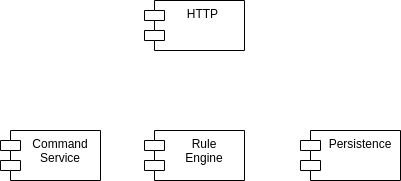
\includegraphics[width=\textwidth,height=\textheight,keepaspectratio]{simple-componentModel}
    \caption{Simple Backend Component Model}
\end{figure}
